\documentclass[oneside]{report}
\usepackage[T1]{fontenc}
\usepackage[utf8]{inputenc}
\usepackage[french]{babel}
\usepackage{graphicx}
\usepackage[margin=2cm]{geometry}
\usepackage{fancyhdr}
\usepackage{changepage}
\usepackage{etoolbox}
\usepackage{xcolor}
\usepackage{listings}
\usepackage{titlesec}

\titleformat{\chapter}[display]
{\normalfont\huge\bfseries}{}{20pt}{\Huge}

\titlespacing*{\chapter}{0pt}{0pt}{0pt}
\graphicspath{{./images/}}

\author{Sylvain COMBRAQUE, Sarah LAMOTTE, Nathan JANCZEWSKI, Léo BERGEROT}

\newcommand\softname{Alohomora\ }
\newcommand{\writecol}[1]{
	\subitem{\textcolor[HTML]{#1}{\# #1}}
}

\patchcmd{\chapter}{plain}{fancy}{}{}


\lstset{
	string=[s]{"}{"},
	stringstyle=\color{blue},
	comment=[l]{:},
	commentstyle=\color{black},
}

\begin{document}

	\begin{titlepage}
		\centering
		
\includegraphics[scale=.5]{logo_large}
		\vspace{5cm}
		{\par\scshape\Huge Documents techniques\par}
		\vspace{5cm}
		{\par Gestionnaire de mot de passes\par}
		{\par Application et API\par}
		\vfill
		\par Contact:
		{\par\small Mr.\ Jerôme CUTRONA \par}
		\par jerome.cutrona@univ-reims.fr\
	\end{titlepage}

	\pagestyle{fancy}
	\fancyhf{}
	\lhead{Documents techniques}
	\rhead{
\includegraphics[scale=.25]{logo_large}}
	\tableofcontents

	\chapter{Informations générales}
	\vspace{2cm}
	\par Les requêtes auront lieu à l'URL "https://alohomora.pw/api/". L'API étant basé sur GraphQL, aucune autre route ne sera à prévoir.\\
	\par Le serveur pourra au choix activer ou désactiver l'inscription publique (N'importe qui peut s'inscrire), l'inscription via API (L'utilisateur ne pourra s'inscrire que depuis le site web), le nombre de requêtes par minutes (éviter un flood de 'getUpdates').\\

	\par Les réponses sont envoyé par le serveur au format json.\\

	\chapter{Diagrammes réseau}
	\vspace{2cm}
	\section{Inscription}{
		\par L'inscription au serveur est effectué via une requête register.\\
		\vspace{.5cm}
		\begin{center}
			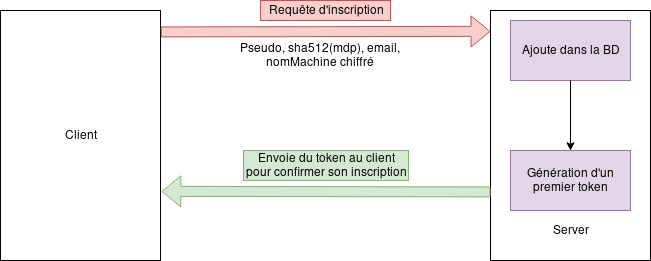
\includegraphics[scale=.5]{reseau_register}
		\end{center}
	}

	\section{Connexion}{
		\par La connexion au serveur permet à l'utilisateur d'obtenir un token lui permettant d'intéragir avec son compte sans que le mot de passe transite. Ce token pourra aussi être révoqué.\\
		\vspace{.5cm}
		\begin{center}
			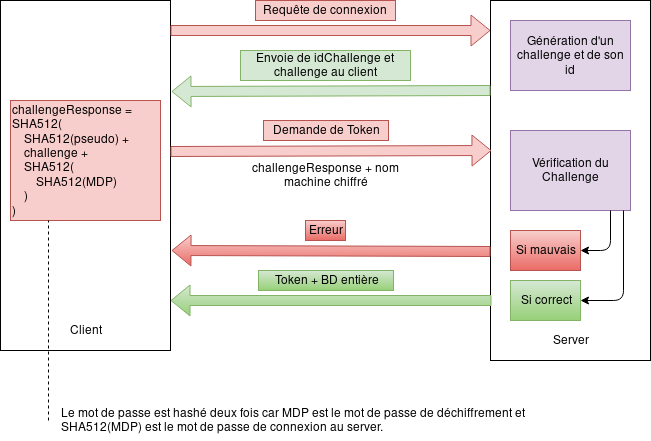
\includegraphics[scale=.5]{reseau_connexion}
		\end{center}
	}

	\section{Récupérer les changements côté serveur}{
		\par Le client peut demander au serveur tous ce qui a changé sur son compte depuis sa dernière mise à jour.
		\par Par défaut, le client peut demander à un interval régulier des mises à jour, cependant le serveur peut refuser et demander au client une synchronisation manuelle via un bouton "Refresh"
		\begin{center}
			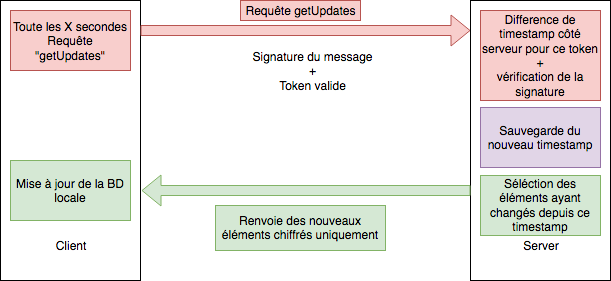
\includegraphics[scale=.5]{reseau_getupdates}
		\end{center}
	}

	\section{Ajout d'un élément}{
		\par Pour ajouter un élément, le client fait une requête en joignant un élément JSON chiffré.
		\par Afin de respecter une cohérence entre les clients, un schéma nécessaire est fourni dans les chapitres suivant de ce document.
		\begin{center}
			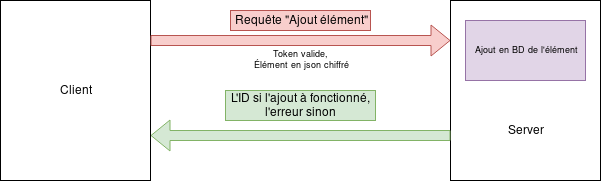
\includegraphics[scale=.5]{reseau_add_elt}
		\end{center}

	}

	\section{Modification ou suppression d'un élément}{
		\par De la même façon que pour ajouter un élément, un client peut le modifier en renvoyant ce dernier et en précisant son ID.
		\par Pour supprimer un élément, le client envoie une requête de modification sans paramètre du contenu.
		\begin{center}
			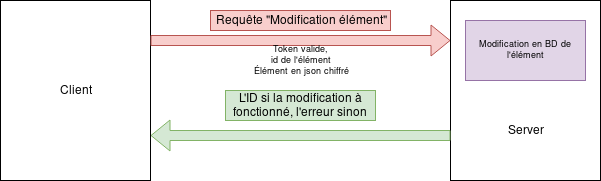
\includegraphics[scale=.5]{reseau_update_elt}
		\end{center}
	}

	\chapter{Client(s)}
	\section{Structuration des données}{
		\subsection{Contenu d'un élément} {
			\vspace{1cm}
			\begin{lstlisting}
				{
					"type": 0,
					"id": 1,
					"name": "Name of the element which will be displayed",
					"customField": "value",
					"customField2": "value"
				}
			\end{lstlisting}
			\vspace{1cm}
			\par Le champ type peut prendre les valeurs 0 dans le cas d'un élément de type "Mot de passe", 1 dans le cas d'un élément de type "Mémo" et 2 dans le cas d'un élément de type "Marque-page".
			\par L'id est un identifiant afin que le client puisse effectuer des requêtes tels que la modification sur un élément.
			\par Le champ nom est le texte affiché quand on souhaite séléctionner un élément afin que l'utilisateur puisse l'identifier.
			\par Après ces champs, dans le cas d'un mot de passe, les autres champs disponibles sont "username", "password" et "url".
			\par Dans le cas d'un mémo le seul champ supplémentaire est un champ "Contenu" qui contiendra le texte du mémo écrite en Markdown.
			\par Enfin, dans le cas d'un marque page, le champ supplémentaire sera "url"
			\par Cependant, des champs personnalisés (Ici représenté par "customfield" et "customfield2") seront ajoutable par l'utilisateur. Il n'y a pas de limite au nombre de champs, l'interface devant donc s'y adapter.
		}
	}
	\section{Sécurité}{
		\begin{itemize}
			\item Lors de l'affichage d'une fiche de mot de passe, il ne doit être visible que si l'utilisateur intéragit avec la textfield.
			\item Un bouton permettant de copier le mot de passe doit être mis à disposition afin que l'utilisateur n'ai pas à afficher son mot de passe obligatoirement.
		\end{itemize}
	}

	\section{Ergonomie}{
		\begin{itemize}
			\item Raccourcis clavier CTRL+C / CTRL+B pour copier le mot de passe ou le nom d'utilisateur
		\end{itemize}
	}


\end{document}
